%Copyright (c) 2004 2005 2006 Atos Origin
%Permission is granted to copy, distribute and/or modify this
%document
%under the terms of the GNU Free Documentation License,
%      Version 1.2
%      or any later version published by the Free Software
%      Foundation;
%      with no Invariant Sections, no Front-Cover
%      Texts, and no Back-Cover
%      Texts.  A copy of the license is
%      included in the section entitled "GNU
%      Free Documentation License".
%
%$Id: eval.tex,v 1.1 2006/02/16 18:21:09 goneri Exp $
\section{Evaluer}
\begin{figure}
\center
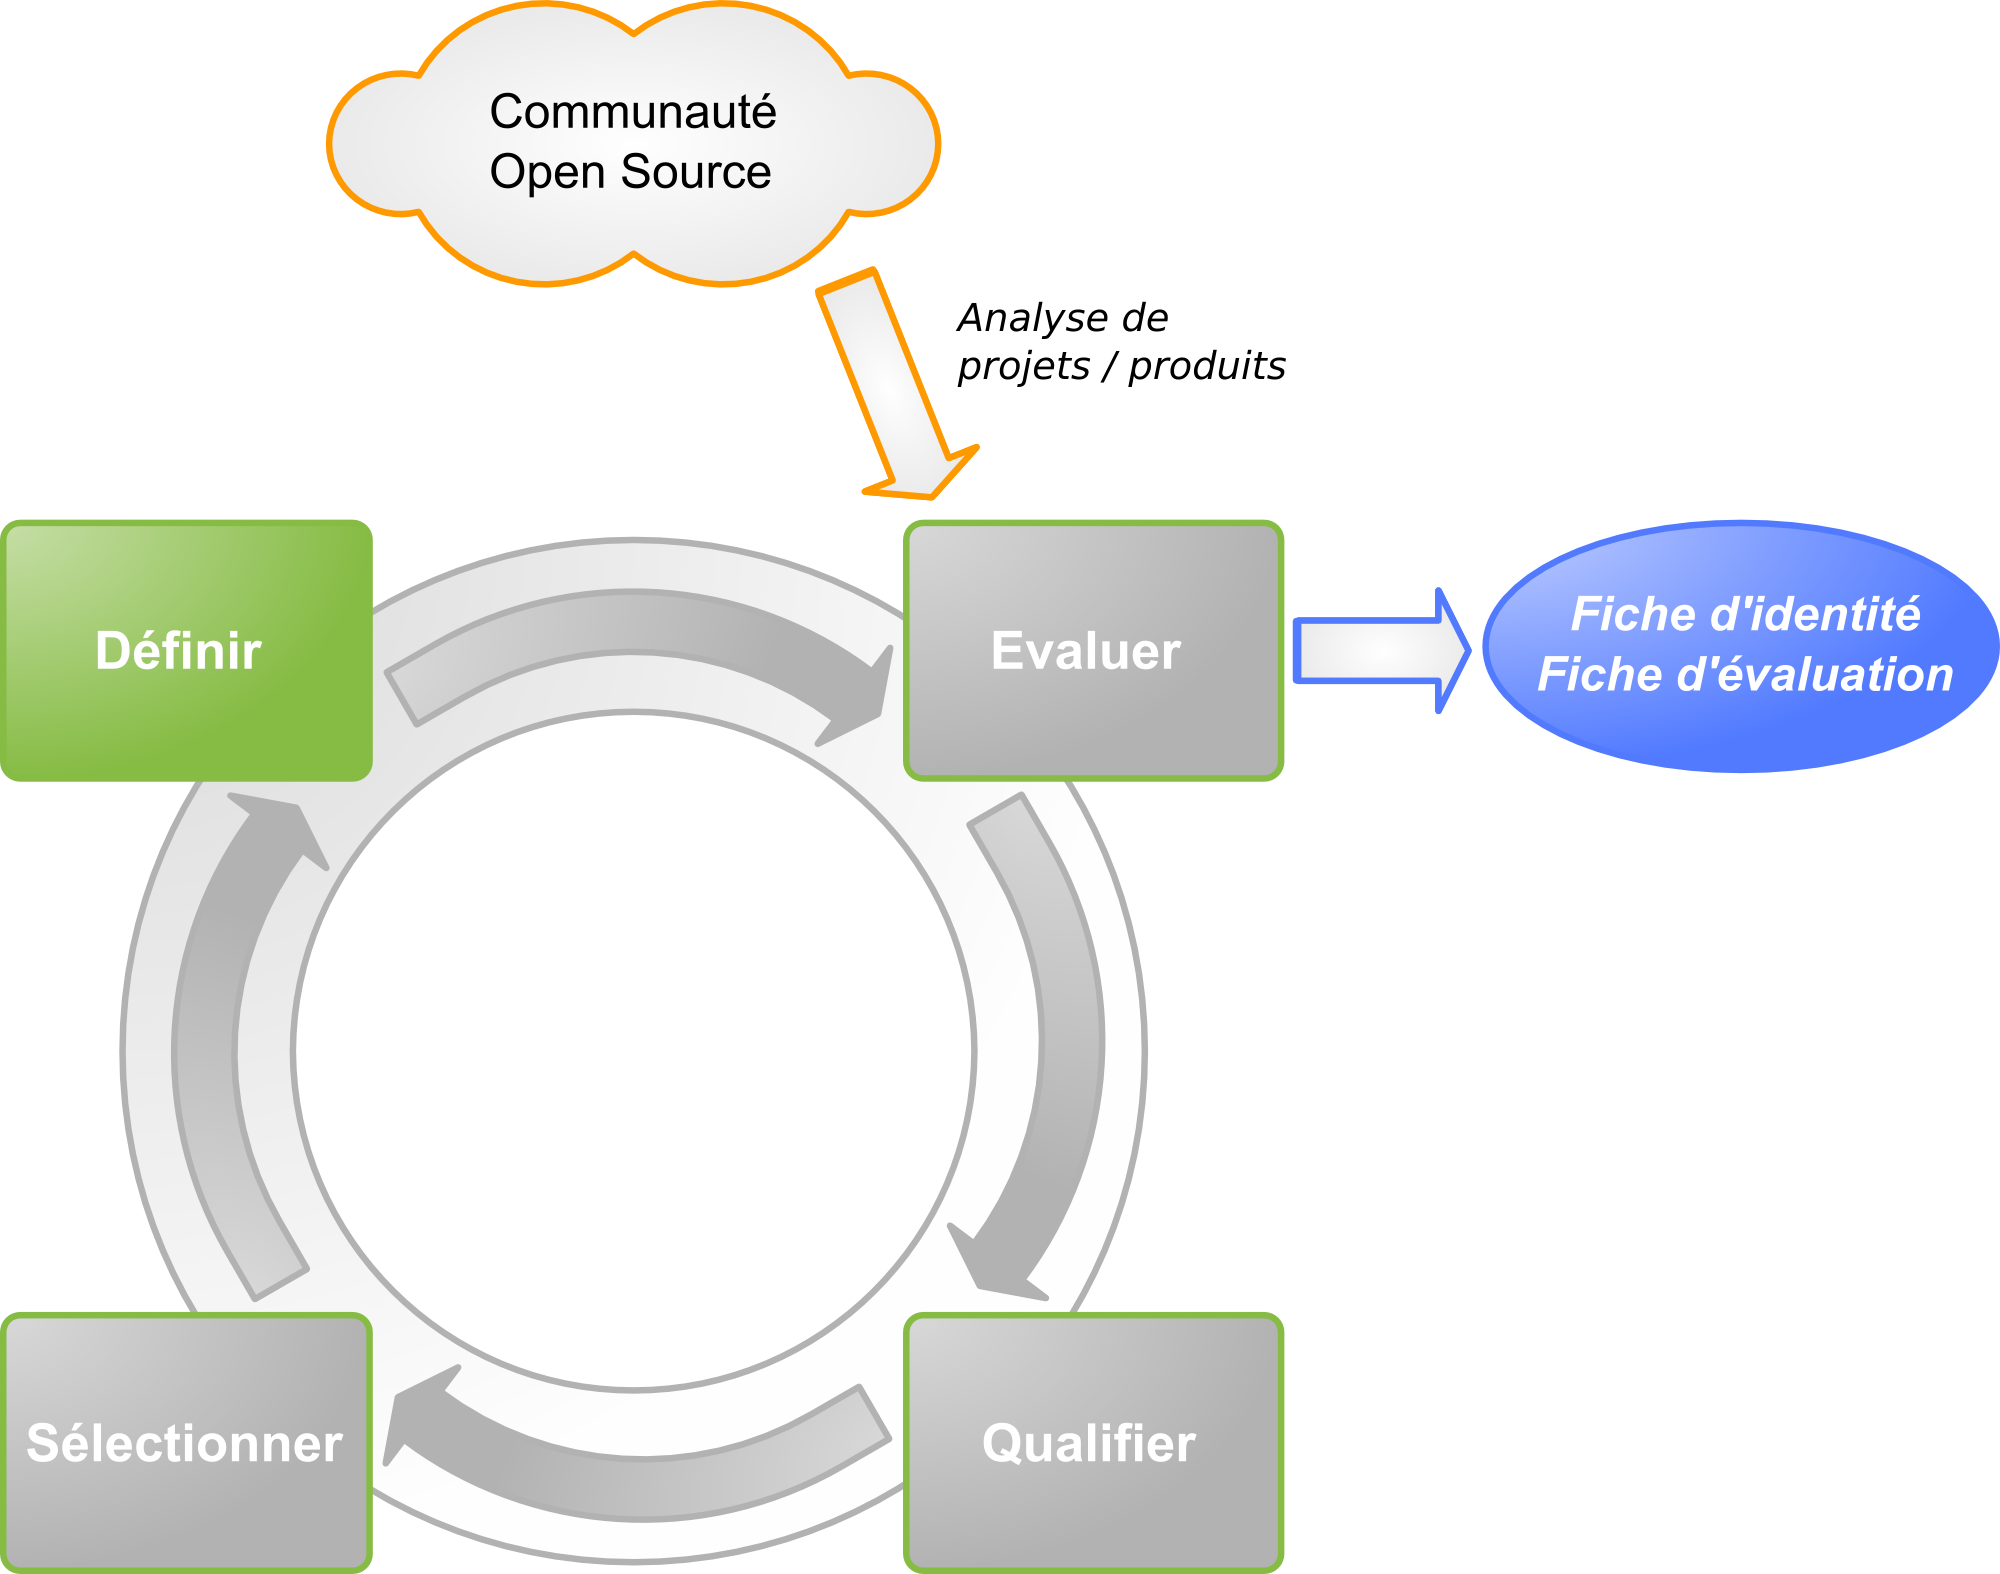
\includegraphics[width=13cm]{images/fr/evaluer}
\caption{�valuer}
\end{figure}


\subsection{Objectif}
L'objectif de cette �tape est de proc�der � l'�valuation des logiciels Open Source.
Elle consiste � r�cup�rer des informations depuis la communaut� Open Source, de mani�re � :

\begin{itemize}
\item Constituer les fiches d'identit� d'un logiciel
\item Constituer sa fiche d'�valuation : noter le logiciel selon des crit�res r�partis
sur trois axes majeurs :
  \begin{itemize}
  \item Couverture fonctionnelle 
  \item Risques du point de vue de l'Utilisateur
  \item Risques du point de vue du Prestataire de services 
  \end{itemize}
\end{itemize}
Ce travail d'�valuation est ins�rable dans une d�marche plus large de veille technologique qui n'est pas d�crite ici dans sa globalit�.

\subsection{Fiche d'identit� de logiciel}
Les donn�es constituant la fiche d'identit� du logiciel sont des donn�es brutes et 
factuelles qui ne sont pas directement not�es mais sur lesquelles se base en partie
la notation des crit�res pr�sent�s plus loin.


Les principaux points de la fiche d'identit� de logiciel sont les suivants :


\subsubsection{Informations g�n�rales}
\begin{itemize}
\item Nom du logiciel
\item R�f�rence, dates de cr�ation et de mise jour de la fiche
\item Auteur de la fiche 
\item Domaine fonctionnel du logiciel 
\item Description succincte du logiciel 
\item Licences auxquelles est soumis le logiciel 
\item URL du site principal du projet Open Source et de d�monstration du logiciel
\item Syst�mes d'exploitation compatibles
\item Origine du fork (si le logiciel provient d'un fork)
\end{itemize}

\subsubsection{Services existants}
\begin{itemize}
\item Documentation
\item Nombre d'offres de support contractuel 
\item Nombre d'offres de prestations de formation
\item Nombre d'offres de prestations de conseil
\end{itemize}

\subsubsection{Aspects fonctionnels et techniques}
\begin{itemize}
\item Technologie(s) d'impl�mentation 
\item Pr� requis techniques 
\item Fonctionnalit�s d�taill�es 
\item Plan de d�veloppement ou � roadmap�
\end{itemize}

\subsubsection{Synth�se}
\begin{itemize}
\item Tendance g�n�rale 
\item Commentaire synth�tique 
\end{itemize}

